\section{Fallbeispiel: Der Zahllauf}\label{chap:paymentrun}

TODO: Umschreiben zu Thomas' Vorschlag!!!


Im Bereich der Geschäftsanwendungen gibt es eine Reihe hochkomplexer Prozesse, die in der IT abgebildet werden.
Einer davon ist der sogenannte Zahllauf, bei dem sich der Anwender eine Liste von offenen Zahlungen erst vorschlagen lässt und anschließend veranlasst.
Dabei spielen die Abhängigkeiten von Zahlungen, Lieferanten und Rabattverträgen eine wichtige Rolle, da sie im Idealfall in einer günstigen Konstellation für das Unternehmen resultieren.

\begin{figure}[ht]
	\centering
  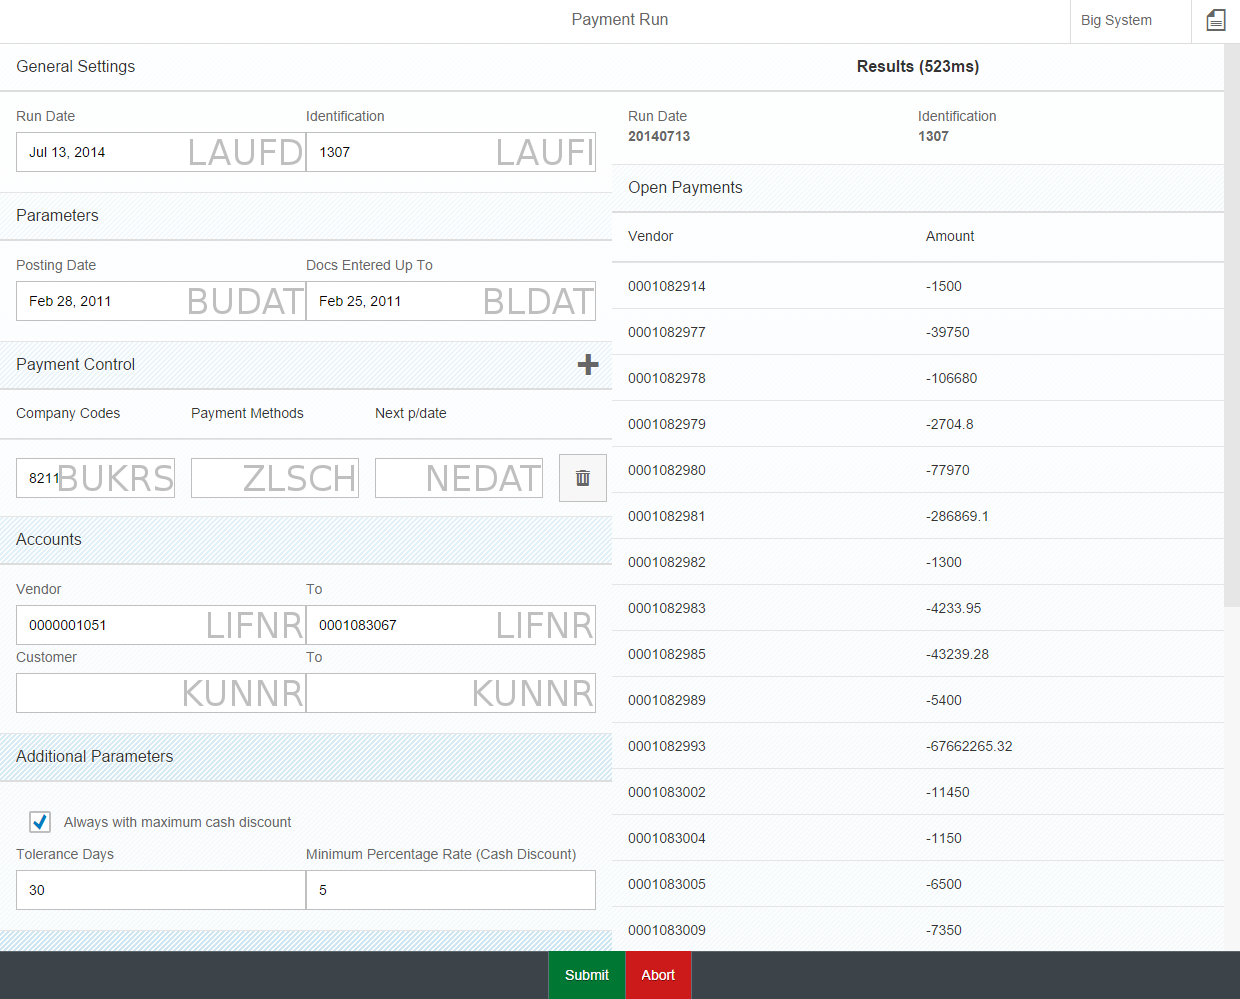
\includegraphics[width=1\textwidth]{figures/paymentrun.png}
	\caption{Eingabemaske des Zahllaufs}
	\label{fig:paymentrun}
\end{figure}

Dementsprechend gibt es viele Einflussfaktoren und Variablen in der Umsetzung des dazugehörigen Algorithmus'.
Dies macht es vor allem dem Entwickler schwer: große Tabellen mit zum Teil kryptischen Feldern und Werten dienen als Grundlage, Zwischenspeicher und Ausgabe.
Da es wichtig ist bereits während der Entwicklung die Performance zu testen, sind sinnvolle Testdaten nötig, die frühzeitig auch die Randfälle der Implementierung aufdecken.

\subsection{Der Einfluss der Eingabe auf die resultierende Query}
Die Eingabemaske des Zahllaufs besteht aus vielen allgemeinen Parametern und einzelnen Suchfeldern für bestimmte Rechnungen.
Neben den Identifikationsmerkmalen für den Lauf, kann ein Zeitbereich festgelegt werden, in dem die Zahlungen liegen.
Anschließend werden in Tabellenform Suchkriterien (Buchungskreise, Zahlmethoden, nächstes Ausführungsdatum) eingeben um Zahlungen herauszufiltern.
Die einzelnen Zellen einer Reihe bilden eine Konjunktion, wobei die Reihen miteinander disjunkt sind.
Komplexität entsteht durch die vielen Möglichkeiten von Eingaben.
So können z.B. Buchungskreise kommasepariert, mittels Klammern als Bereich oder beides kombiniert angeben werden.
Die Zahlmethoden werden mit Großbuchstaben abgekürzt und aneinander gereiht um mehrere Methoden zuzulassen.
Schlussendlich können noch Filter nach Kunden- und Lieferanten-Nummern angegeben werden, wobei hier einzelne oder Bereichsangaben möglich sind, wie man im (bereits im Kapitel \ref{sec:dependencydetection} gezeigten) Code-Beispiel \ref{lst:paymentrun} erkennen kann.

\begin{lstlisting}[caption={Mehrere Möglichkeiten des Auswahl anhand von Kundennummern}, label={lst:paymentrun}, language=JavaScript]
	var stmt = "SELECT BSIK.BUKRS, BSIK.LIFNR, LFA1.CONFS
	FROM CUSTOMER.BSIK LEFT OUTER JOIN CUSTOMER.LFA1
	ON BSIK.MANDT = LFA1.MANDT AND BSIK.LIFNR = LFA1.LIFNR
	WHERE ";
	if(customer && !customerTo){
		stmt += "LFA1.KUNNR = '" + customer + "'";
	}
	if(customer && customerTo){
		stmt += "LFA1.KUNNR BETWEEN '" + customer +
						"' AND '" + customerTo + "'" ;
	}
\end{lstlisting}

Diese Variabilität in der Eingabemaske schlägt sich auch auf das resultierende SQL-Statement nieder, dessen Aussehen, Komplexität und Laufzeit durch die optionalen Parameter bestimmt wird, weshalb passende Testdaten für den Entwickler wichtig sind.

\subsection{Passende Vorschl{\"a}ge f{\"u}r das Testen des Zahllauf-Programms}
Skizzieren welche Vorschläge der Algorithmus für das Programm liefert

- Vergleich von meinem Ansatz mit Brute-Force beim Fallbeispiel
  - Evaluiering: Zeit-Aufwand vs. bessere Ergebnisse
  - Betrachtung von Datum-Feldern